\documentclass[11pt,a4paper]{amsart}

\usepackage[utf8]{inputenc}

\usepackage{url}

%\usepackage{makeidx}

\numberwithin{equation}{section}
\newtheorem{theorem}{Theorem}[section]
\newtheorem*{theorem*}{Theorem}
\newtheorem{lemma}[theorem]{Lemma}
\newtheorem{prop}[theorem]{Proposition}
\newtheorem{corollary}[theorem]{Corollary}
\theoremstyle{definition}
\newtheorem{definition}[theorem]{Definition}
\newtheorem{claim}[theorem]{Claim}
\newtheorem{problem}[theorem]{Problem}
\newtheorem{remark}[theorem]{Remark}
\newtheorem{fact}[theorem]{Fact}
\newtheorem{example}[theorem]{Example}
\newtheorem{observation}[theorem]{Observation}
\newtheorem{conjecture}[theorem]{Conjecture}

\usepackage{graphicx}

\newcommand{\ZZ}{{\mathbb{Z}}}
\newcommand{\QQ}{{\mathbb{Q}}}
\newcommand{\RR}{{\mathbb{R}}}
\newcommand{\CC}{{\mathbb{C}}}
\newcommand{\NN}{{\mathbb{N}}}
\newcommand{\KK}{{\mathbb{K}}}

%\documentclass[11pt,a4paper]{amsart}

\usepackage[utf8]{inputenc}

\usepackage{url}

%\usepackage{makeidx}

\numberwithin{equation}{section}
\newtheorem{theorem}{Theorem}[section]
\newtheorem*{theorem*}{Theorem}
\newtheorem{lemma}[theorem]{Lemma}
\newtheorem{prop}[theorem]{Proposition}
\newtheorem{corollary}[theorem]{Corollary}
\theoremstyle{definition}
\newtheorem{definition}[theorem]{Definition}
\newtheorem{claim}[theorem]{Claim}
\newtheorem{problem}[theorem]{Problem}
\newtheorem{remark}[theorem]{Remark}
\newtheorem{fact}[theorem]{Fact}
\newtheorem{example}[theorem]{Example}
\newtheorem{observation}[theorem]{Observation}
\newtheorem{conjecture}[theorem]{Conjecture}



\newcommand{\ZZ}{{\mathbb{Z}}}
\newcommand{\QQ}{{\mathbb{Q}}}
\newcommand{\RR}{{\mathbb{R}}}
\newcommand{\CC}{{\mathbb{C}}}
\newcommand{\NN}{{\mathbb{N}}}
\newcommand{\KK}{{\mathbb{K}}}

%\documentclass[11pt,a4paper]{amsart}

\usepackage[utf8]{inputenc}

\usepackage{url}

%\usepackage{makeidx}

\numberwithin{equation}{section}
\newtheorem{theorem}{Theorem}[section]
\newtheorem*{theorem*}{Theorem}
\newtheorem{lemma}[theorem]{Lemma}
\newtheorem{prop}[theorem]{Proposition}
\newtheorem{corollary}[theorem]{Corollary}
\theoremstyle{definition}
\newtheorem{definition}[theorem]{Definition}
\newtheorem{claim}[theorem]{Claim}
\newtheorem{problem}[theorem]{Problem}
\newtheorem{remark}[theorem]{Remark}
\newtheorem{fact}[theorem]{Fact}
\newtheorem{example}[theorem]{Example}
\newtheorem{observation}[theorem]{Observation}
\newtheorem{conjecture}[theorem]{Conjecture}



\newcommand{\ZZ}{{\mathbb{Z}}}
\newcommand{\QQ}{{\mathbb{Q}}}
\newcommand{\RR}{{\mathbb{R}}}
\newcommand{\CC}{{\mathbb{C}}}
\newcommand{\NN}{{\mathbb{N}}}
\newcommand{\KK}{{\mathbb{K}}}

%\documentclass[11pt,a4paper]{amsart}

\usepackage[utf8]{inputenc}

\usepackage{url}

%\usepackage{makeidx}

\numberwithin{equation}{section}
\newtheorem{theorem}{Theorem}[section]
\newtheorem*{theorem*}{Theorem}
\newtheorem{lemma}[theorem]{Lemma}
\newtheorem{prop}[theorem]{Proposition}
\newtheorem{corollary}[theorem]{Corollary}
\theoremstyle{definition}
\newtheorem{definition}[theorem]{Definition}
\newtheorem{claim}[theorem]{Claim}
\newtheorem{problem}[theorem]{Problem}
\newtheorem{remark}[theorem]{Remark}
\newtheorem{fact}[theorem]{Fact}
\newtheorem{example}[theorem]{Example}
\newtheorem{observation}[theorem]{Observation}
\newtheorem{conjecture}[theorem]{Conjecture}



\newcommand{\ZZ}{{\mathbb{Z}}}
\newcommand{\QQ}{{\mathbb{Q}}}
\newcommand{\RR}{{\mathbb{R}}}
\newcommand{\CC}{{\mathbb{C}}}
\newcommand{\NN}{{\mathbb{N}}}
\newcommand{\KK}{{\mathbb{K}}}

%\input{definitions}
\makeindex
\begin{document}
\title{Definitions of terms used in the SDEval Project}
\author{Albert Heinle}


\maketitle
\section{Definitions}

\begin{definition}[Task]
\label{def:Task}
\index{Task}
A task is always associated to a certain computation problem (see
Definition \ref{def:ComputationProblem}). A task contains a list of
SD-Tables (see Definition \ref{def:SD-Table}), that contain entries
that are suitable as input for the associated computation problem.

From those SD-Tables, a task contains a set of problem instances (see
Definition \ref{def:ProblemInstance}). Additionally, a task contains a
set of computer algebra systems (see Definition
\ref{def:computeralgebrasystem}), that provide algorithms for solving the
associated computation problem. Every set in a task is not
empty. Furthermore, a task has a name.
\end{definition}

\begin{example}[Task]
Let us call a task \texttt{xyz}, and let its associated computation
problem be \texttt{GB\_Z\_lp}.

This is an entry in the Symbolic-Data
table \texttt{COMP} and represents the commutative Gr\"obner basis
computation in a commutative ring using the lexicographical ordering
and given generators that have coefficients in $\ZZ$.

The only existing SD-Table, that provides an entries that can be used
as inputs for the Gr\"obner basis algorithms, is meanwhile
\texttt{INTPS} (see Symbolic-Data). From this table, we choose as one
of our problem instances the instance \texttt{Amrhein}. A computer
algebra system, that provides an algorithm for \texttt{GB\_Z\_lp} is
for example \textsc{Singular}.
\end{example}

\begin{definition}[Computation Problem]
\label{def:ComputationProblem}
\index{Computation Problem}
A computation problem is a problem, which is specified in the SD-Table
(see Definition \ref{def:SD-Table})
\texttt{COMP} of the Symbolic Data project. In the context of
\textsc{SDEval} we are using it to specify which computations
we want to perform on certain problem instances (see Definition
\ref{def:ProblemInstance}), resp. which algorithm shall be used.
\end{definition}

\begin{example}[Computation Problem]
 A computation
problem is for example \texttt{GB\_Z\_lp}.

This is an entry in the SD-Table
table \texttt{COMP} and represents the commutative Gr\"obner basis
computation in a commutative ring using the lexicographical ordering
and given generators that have coefficients in $\ZZ$.
\end{example}

\begin{definition}
\label{def:ProblemInstance}
\index{Problem Instance}
A problem instance is in our context a representation -- specified by
Symbolic-Data -- of a concrete input for suitable algorithms. Suitable
means that the entries for the chosen algorithms can be read from this
problem instance. A problem instance is always contained in a SD-Table
(see Definition \ref{def:SD-Table})
\end{definition}

\begin{example}[Problem Instance]
  A problem instance is for example the entry \texttt{Amrhein} in the
  SD-Table \texttt{INTPS}. It contains variables and a basis of
  polynomials, and those can be used for Gr\"obner basis computations,
  for example.
\end{example}

\begin{definition}[SD-Table]
\label{def:SD-Table}
\index{SD-Table}
A SD-Table denotes the folder structure of a chosen subfolder in the
\texttt{XMLRessources} folder in the Symbolic-Data project.
\end{definition}

\begin{example}[SD-Table]
There are several folders in \texttt{XMLRessources}. Some examples:
\begin{itemize}
   \item \texttt{INTPS}
   \item \texttt{COMP}
   \item \texttt{ModPS}
   \item \texttt{CAS}
\end{itemize}
\end{example}

\begin{definition}[Computer Algebra System]
\label{def:computeralgebrasystem}
\index{Computer Algebra System}
  A computer algebra system is a program, described by an entry in the
  SD-Table \texttt{CAS} (see Definition \ref{def:SD-Table}). It
  provides algorithms to solve different computation problems (see
  Definition \ref{def:ComputationProblem}).
\end{definition}

\begin{example}[Computer Algebra System]
  \textsc{Singular} (\url{http://www.singular.uni-kl.de/}) is for example a computer algebra system.
\end{example}

\begin{definition}[Taskfolder]
  \label{def:TaskFolder}
  \index{Taskfolder}
  A taskfolder is always associated to exactly one task (see
  Definition \ref{def:Task}). It contains
  \begin{itemize}
    \item The task itself
    \item For every problem instance (see Definition \ref{def:ProblemInstance}) and for every computer algebra
      system (see Definition \ref{def:computeralgebrasystem}) the taskfolder contains one executable file, that
      contains the calculation steps for the calculation of the
      computation problem (see Definition
      \ref{def:ComputationProblem}).
    \item An executable file \texttt{runTasks.py} and all needed
      modules (see Definition \ref{def:module}) of this file.
    \item The machine settings (see Definition
      \ref{def:MachineSettings}) for the target machine (see
      Definition \ref{def:TargetMachine}) of the task
  \end{itemize}
  It serves the purpose to be exported as a single folder to a target
  machine, where the calculations shall be run at.
\end{definition}

\begin{example}[Taskfolder]
  In order to have an example of an taskfolder, just run
  \texttt{create\_tasks[\_gui].py}, and the folder that is created in
  the end, that is an taskfolder.
\end{example}

\begin{definition}[Module]
  \label{def:module}
  \index{module}
  A module is a collection of executable code of a certain programming/script-language.
\end{definition}

\begin{example}[Module]
  In the SDEval project, there is for example a module called

  \texttt{classes.probleminstances}.

It contains representations as
  classes of different types of problem instances.
\end{example}

\begin{definition}[Machine Settings]
\label{def:MachineSettings}
\index{Machine Settings}
Machine settings is a collection of machine-specific constants of the
target machine (see Definition \ref{def:TargetMachine}); Those are:
\begin{itemize}
  \item For every computer algebra system the command to execute it on
    the target machine.
  \item The command for the time measurement (time command, see
    Definition \ref{def:TimeCommand}) on the target machine with the
    desired options of the user.
  \item Optional, it can contain further entries.
\end{itemize}
\end{definition}

\begin{example}[Machine Settings]
  The command for time measurement is on every \texttt{UNIX}-like
  machine simply \texttt{time}. The command to run e.g. version 15 of
  \textsc{Maple} on a machine known to the author is \texttt{maple15}.
\end{example}

\begin{definition}[Target Machine]
  \label{def:TargetMachine}
  \index{Target Machine}
  A target machine is the computer on which in the end the
  computations for a specific task (see Definition \ref{def:Task})
  will take place. In our choices of words we assume in general, that
  it has a \texttt{UNIX}-like operating system installed. There must
  be a time command available on that machine (see Definition \ref{def:TimeCommand}).
\end{definition}

\begin{definition}[Time Command]
  \label{def:TimeCommand}
  \index{Time Command}
  A time command is a tool for time measurement. On \texttt{UNIX}-like
  operating systems it is e.g. the command \texttt{time}.

  In the context of SDEval we need that this time command is able to produce its
  output in the IEEE Std 1003.2-1992 (``POSIX.2'') described way. On
  \texttt{UNIX}-machines, it is achieved by adding the option
  \texttt{-p} to the command.
\end{definition}

\begin{example}[Time Command]
  For example, on a mac, this is how the time command works:
  \begin{verbatim}
$ time -p echo "Hello"
Hello
real 0.00
user 0.00
sys 0.00
 \end{verbatim}
\end{example}

\begin{definition}[Proceedings]
\label{def:Proceedings}
\index{Proceedings}
Proceedings contain information about the status of the execution of
the files in the task folder (see Definition
\ref{def:TaskFolder}). For the status, there are the following
options:
\begin{itemize}
  \item RUNNING     -- The file is running
  \item WAITING      -- The file is waiting for its execution
  \item COMPLETED -- The execution of the file is finished
  \item ERROR          -- An Error occured
\end{itemize}
During the execution, there will always be an XML and an HTML file
written visualizing the current proceedings.
\end{definition}

\begin{example}[Proceedings]
Let us take the entry \texttt{Amrhein} of the \texttt{INTPS} table and
let the computer algebra systems \textsc{Singular} and \textsc{Maple}
be chosen for the computation of a Gr\"obner basis of those
systems.

In the beginning, both execution files (i.e. for \textsc{Singular} and
\textsc{Maple}) are WAITING. If one of the files is executed on its
computer algebra system, it has the status RUNNING, and when the
computation is completed, the status will change to COMPLETED.
\end{example}

\begin{definition}[Resulting File]
\label{def:ResultingFile}
\index{Resulting File}
During the execution of the files in an task folder (see Definition
\ref{def:TaskFolder}), there are always resulting files containing the
output of the computer algebra system (see Definition
\ref{def:computeralgebrasystem}) and the time command (see Definition \ref{def:TimeCommand}).
\end{definition}

\begin{example}[Resulting File]
A resulting file after executing some singular commands has for
example the following form:
\begin{verbatim}
                     SINGULAR                                 /
 A Computer Algebra System for Polynomial Computations       /   version 3-1-5
                                                           0<
 by: W. Decker, G.-M. Greuel, G. Pfister, H. Schoenemann     \   Jul 2012
FB Mathematik der Universitaet, D-67653 Kaiserslautern        \
a2+a+2bf+2ce+d2,
2ab+b+2cf+2de,
2ac+b2+c+2df+e2,
2ad+2bc+d+2ef,
2ae+2bd+c2+e+f2,
2af+2be+2cd+f

$Bye.
real 0.53
user 0.01
sys 0.01
\end{verbatim}
\end{example}

\printindex

\end{document}

\makeindex
\begin{document}
\title{Definitions of terms used in the SDEval Project}
\author{Albert Heinle}


\maketitle
\section{Definitions}

\begin{definition}[Task]
\label{def:Task}
\index{Task}
A task is always associated to a certain computation problem (see
Definition \ref{def:ComputationProblem}). A task contains a list of
SD-Tables (see Definition \ref{def:SD-Table}), that contain entries
that are suitable as input for the associated computation problem.

From those SD-Tables, a task contains a set of problem instances (see
Definition \ref{def:ProblemInstance}). Additionally, a task contains a
set of computer algebra systems (see Definition
\ref{def:computeralgebrasystem}), that provide algorithms for solving the
associated computation problem. Every set in a task is not
empty. Furthermore, a task has a name.
\end{definition}

\begin{example}[Task]
Let us call a task \texttt{xyz}, and let its associated computation
problem be \texttt{GB\_Z\_lp}.

This is an entry in the Symbolic-Data
table \texttt{COMP} and represents the commutative Gr\"obner basis
computation in a commutative ring using the lexicographical ordering
and given generators that have coefficients in $\ZZ$.

The only existing SD-Table, that provides an entries that can be used
as inputs for the Gr\"obner basis algorithms, is meanwhile
\texttt{INTPS} (see Symbolic-Data). From this table, we choose as one
of our problem instances the instance \texttt{Amrhein}. A computer
algebra system, that provides an algorithm for \texttt{GB\_Z\_lp} is
for example \textsc{Singular}.
\end{example}

\begin{definition}[Computation Problem]
\label{def:ComputationProblem}
\index{Computation Problem}
A computation problem is a problem, which is specified in the SD-Table
(see Definition \ref{def:SD-Table})
\texttt{COMP} of the Symbolic Data project. In the context of
\textsc{SDEval} we are using it to specify which computations
we want to perform on certain problem instances (see Definition
\ref{def:ProblemInstance}), resp. which algorithm shall be used.
\end{definition}

\begin{example}[Computation Problem]
 A computation
problem is for example \texttt{GB\_Z\_lp}.

This is an entry in the SD-Table
table \texttt{COMP} and represents the commutative Gr\"obner basis
computation in a commutative ring using the lexicographical ordering
and given generators that have coefficients in $\ZZ$.
\end{example}

\begin{definition}
\label{def:ProblemInstance}
\index{Problem Instance}
A problem instance is in our context a representation -- specified by
Symbolic-Data -- of a concrete input for suitable algorithms. Suitable
means that the entries for the chosen algorithms can be read from this
problem instance. A problem instance is always contained in a SD-Table
(see Definition \ref{def:SD-Table})
\end{definition}

\begin{example}[Problem Instance]
  A problem instance is for example the entry \texttt{Amrhein} in the
  SD-Table \texttt{INTPS}. It contains variables and a basis of
  polynomials, and those can be used for Gr\"obner basis computations,
  for example.
\end{example}

\begin{definition}[SD-Table]
\label{def:SD-Table}
\index{SD-Table}
A SD-Table denotes the folder structure of a chosen subfolder in the
\texttt{XMLRessources} folder in the Symbolic-Data project.
\end{definition}

\begin{example}[SD-Table]
There are several folders in \texttt{XMLRessources}. Some examples:
\begin{itemize}
   \item \texttt{INTPS}
   \item \texttt{COMP}
   \item \texttt{ModPS}
   \item \texttt{CAS}
\end{itemize}
\end{example}

\begin{definition}[Computer Algebra System]
\label{def:computeralgebrasystem}
\index{Computer Algebra System}
  A computer algebra system is a program, described by an entry in the
  SD-Table \texttt{CAS} (see Definition \ref{def:SD-Table}). It
  provides algorithms to solve different computation problems (see
  Definition \ref{def:ComputationProblem}).
\end{definition}

\begin{example}[Computer Algebra System]
  \textsc{Singular} (\url{http://www.singular.uni-kl.de/}) is for example a computer algebra system.
\end{example}

\begin{definition}[Taskfolder]
  \label{def:TaskFolder}
  \index{Taskfolder}
  A taskfolder is always associated to exactly one task (see
  Definition \ref{def:Task}). It contains
  \begin{itemize}
    \item The task itself
    \item For every problem instance (see Definition \ref{def:ProblemInstance}) and for every computer algebra
      system (see Definition \ref{def:computeralgebrasystem}) the taskfolder contains one executable file, that
      contains the calculation steps for the calculation of the
      computation problem (see Definition
      \ref{def:ComputationProblem}).
    \item An executable file \texttt{runTasks.py} and all needed
      modules (see Definition \ref{def:module}) of this file.
    \item The machine settings (see Definition
      \ref{def:MachineSettings}) for the target machine (see
      Definition \ref{def:TargetMachine}) of the task
  \end{itemize}
  It serves the purpose to be exported as a single folder to a target
  machine, where the calculations shall be run at.
\end{definition}

\begin{example}[Taskfolder]
  In order to have an example of an taskfolder, just run
  \texttt{create\_tasks[\_gui].py}, and the folder that is created in
  the end, that is an taskfolder.
\end{example}

\begin{definition}[Module]
  \label{def:module}
  \index{module}
  A module is a collection of executable code of a certain programming/script-language.
\end{definition}

\begin{example}[Module]
  In the SDEval project, there is for example a module called

  \texttt{classes.probleminstances}.

It contains representations as
  classes of different types of problem instances.
\end{example}

\begin{definition}[Machine Settings]
\label{def:MachineSettings}
\index{Machine Settings}
Machine settings is a collection of machine-specific constants of the
target machine (see Definition \ref{def:TargetMachine}); Those are:
\begin{itemize}
  \item For every computer algebra system the command to execute it on
    the target machine.
  \item The command for the time measurement (time command, see
    Definition \ref{def:TimeCommand}) on the target machine with the
    desired options of the user.
  \item Optional, it can contain further entries.
\end{itemize}
\end{definition}

\begin{example}[Machine Settings]
  The command for time measurement is on every \texttt{UNIX}-like
  machine simply \texttt{time}. The command to run e.g. version 15 of
  \textsc{Maple} on a machine known to the author is \texttt{maple15}.
\end{example}

\begin{definition}[Target Machine]
  \label{def:TargetMachine}
  \index{Target Machine}
  A target machine is the computer on which in the end the
  computations for a specific task (see Definition \ref{def:Task})
  will take place. In our choices of words we assume in general, that
  it has a \texttt{UNIX}-like operating system installed. There must
  be a time command available on that machine (see Definition \ref{def:TimeCommand}).
\end{definition}

\begin{definition}[Time Command]
  \label{def:TimeCommand}
  \index{Time Command}
  A time command is a tool for time measurement. On \texttt{UNIX}-like
  operating systems it is e.g. the command \texttt{time}.

  In the context of SDEval we need that this time command is able to produce its
  output in the IEEE Std 1003.2-1992 (``POSIX.2'') described way. On
  \texttt{UNIX}-machines, it is achieved by adding the option
  \texttt{-p} to the command.
\end{definition}

\begin{example}[Time Command]
  For example, on a mac, this is how the time command works:
  \begin{verbatim}
$ time -p echo "Hello"
Hello
real 0.00
user 0.00
sys 0.00
 \end{verbatim}
\end{example}

\begin{definition}[Proceedings]
\label{def:Proceedings}
\index{Proceedings}
Proceedings contain information about the status of the execution of
the files in the task folder (see Definition
\ref{def:TaskFolder}). For the status, there are the following
options:
\begin{itemize}
  \item RUNNING     -- The file is running
  \item WAITING      -- The file is waiting for its execution
  \item COMPLETED -- The execution of the file is finished
  \item ERROR          -- An Error occured
\end{itemize}
During the execution, there will always be an XML and an HTML file
written visualizing the current proceedings.
\end{definition}

\begin{example}[Proceedings]
Let us take the entry \texttt{Amrhein} of the \texttt{INTPS} table and
let the computer algebra systems \textsc{Singular} and \textsc{Maple}
be chosen for the computation of a Gr\"obner basis of those
systems.

In the beginning, both execution files (i.e. for \textsc{Singular} and
\textsc{Maple}) are WAITING. If one of the files is executed on its
computer algebra system, it has the status RUNNING, and when the
computation is completed, the status will change to COMPLETED.
\end{example}

\begin{definition}[Resulting File]
\label{def:ResultingFile}
\index{Resulting File}
During the execution of the files in an task folder (see Definition
\ref{def:TaskFolder}), there are always resulting files containing the
output of the computer algebra system (see Definition
\ref{def:computeralgebrasystem}) and the time command (see Definition \ref{def:TimeCommand}).
\end{definition}

\begin{example}[Resulting File]
A resulting file after executing some singular commands has for
example the following form:
\begin{verbatim}
                     SINGULAR                                 /
 A Computer Algebra System for Polynomial Computations       /   version 3-1-5
                                                           0<
 by: W. Decker, G.-M. Greuel, G. Pfister, H. Schoenemann     \   Jul 2012
FB Mathematik der Universitaet, D-67653 Kaiserslautern        \
a2+a+2bf+2ce+d2,
2ab+b+2cf+2de,
2ac+b2+c+2df+e2,
2ad+2bc+d+2ef,
2ae+2bd+c2+e+f2,
2af+2be+2cd+f

$Bye.
real 0.53
user 0.01
sys 0.01
\end{verbatim}
\end{example}

\printindex

\end{document}

\makeindex
\begin{document}
\title{Definitions of terms used in the SDEval Project}
\author{Albert Heinle}


\maketitle
\section{Definitions}

\begin{definition}[Task]
\label{def:Task}
\index{Task}
A task is always associated to a certain computation problem (see
Definition \ref{def:ComputationProblem}). A task contains a list of
SD-Tables (see Definition \ref{def:SD-Table}), that contain entries
that are suitable as input for the associated computation problem.

From those SD-Tables, a task contains a set of problem instances (see
Definition \ref{def:ProblemInstance}). Additionally, a task contains a
set of computer algebra systems (see Definition
\ref{def:computeralgebrasystem}), that provide algorithms for solving the
associated computation problem. Every set in a task is not
empty. Furthermore, a task has a name.
\end{definition}

\begin{example}[Task]
Let us call a task \texttt{xyz}, and let its associated computation
problem be \texttt{GB\_Z\_lp}.

This is an entry in the Symbolic-Data
table \texttt{COMP} and represents the commutative Gr\"obner basis
computation in a commutative ring using the lexicographical ordering
and given generators that have coefficients in $\ZZ$.

The only existing SD-Table, that provides an entries that can be used
as inputs for the Gr\"obner basis algorithms, is meanwhile
\texttt{INTPS} (see Symbolic-Data). From this table, we choose as one
of our problem instances the instance \texttt{Amrhein}. A computer
algebra system, that provides an algorithm for \texttt{GB\_Z\_lp} is
for example \textsc{Singular}.
\end{example}

\begin{definition}[Computation Problem]
\label{def:ComputationProblem}
\index{Computation Problem}
A computation problem is a problem, which is specified in the SD-Table
(see Definition \ref{def:SD-Table})
\texttt{COMP} of the Symbolic Data project. In the context of
\textsc{SDEval} we are using it to specify which computations
we want to perform on certain problem instances (see Definition
\ref{def:ProblemInstance}), resp. which algorithm shall be used.
\end{definition}

\begin{example}[Computation Problem]
 A computation
problem is for example \texttt{GB\_Z\_lp}.

This is an entry in the SD-Table
table \texttt{COMP} and represents the commutative Gr\"obner basis
computation in a commutative ring using the lexicographical ordering
and given generators that have coefficients in $\ZZ$.
\end{example}

\begin{definition}
\label{def:ProblemInstance}
\index{Problem Instance}
A problem instance is in our context a representation -- specified by
Symbolic-Data -- of a concrete input for suitable algorithms. Suitable
means that the entries for the chosen algorithms can be read from this
problem instance. A problem instance is always contained in a SD-Table
(see Definition \ref{def:SD-Table})
\end{definition}

\begin{example}[Problem Instance]
  A problem instance is for example the entry \texttt{Amrhein} in the
  SD-Table \texttt{INTPS}. It contains variables and a basis of
  polynomials, and those can be used for Gr\"obner basis computations,
  for example.
\end{example}

\begin{definition}[SD-Table]
\label{def:SD-Table}
\index{SD-Table}
A SD-Table denotes the folder structure of a chosen subfolder in the
\texttt{XMLRessources} folder in the Symbolic-Data project.
\end{definition}

\begin{example}[SD-Table]
There are several folders in \texttt{XMLRessources}. Some examples:
\begin{itemize}
   \item \texttt{INTPS}
   \item \texttt{COMP}
   \item \texttt{ModPS}
   \item \texttt{CAS}
\end{itemize}
\end{example}

\begin{definition}[Computer Algebra System]
\label{def:computeralgebrasystem}
\index{Computer Algebra System}
  A computer algebra system is a program, described by an entry in the
  SD-Table \texttt{CAS} (see Definition \ref{def:SD-Table}). It
  provides algorithms to solve different computation problems (see
  Definition \ref{def:ComputationProblem}).
\end{definition}

\begin{example}[Computer Algebra System]
  \textsc{Singular} (\url{http://www.singular.uni-kl.de/}) is for example a computer algebra system.
\end{example}

\begin{definition}[Taskfolder]
  \label{def:TaskFolder}
  \index{Taskfolder}
  A taskfolder is always associated to exactly one task (see
  Definition \ref{def:Task}). It contains
  \begin{itemize}
    \item The task itself
    \item For every problem instance (see Definition \ref{def:ProblemInstance}) and for every computer algebra
      system (see Definition \ref{def:computeralgebrasystem}) the taskfolder contains one executable file, that
      contains the calculation steps for the calculation of the
      computation problem (see Definition
      \ref{def:ComputationProblem}).
    \item An executable file \texttt{runTasks.py} and all needed
      modules (see Definition \ref{def:module}) of this file.
    \item The machine settings (see Definition
      \ref{def:MachineSettings}) for the target machine (see
      Definition \ref{def:TargetMachine}) of the task
  \end{itemize}
  It serves the purpose to be exported as a single folder to a target
  machine, where the calculations shall be run at.
\end{definition}

\begin{example}[Taskfolder]
  In order to have an example of an taskfolder, just run
  \texttt{create\_tasks[\_gui].py}, and the folder that is created in
  the end, that is an taskfolder.
\end{example}

\begin{definition}[Module]
  \label{def:module}
  \index{module}
  A module is a collection of executable code of a certain programming/script-language.
\end{definition}

\begin{example}[Module]
  In the SDEval project, there is for example a module called

  \texttt{classes.probleminstances}.

It contains representations as
  classes of different types of problem instances.
\end{example}

\begin{definition}[Machine Settings]
\label{def:MachineSettings}
\index{Machine Settings}
Machine settings is a collection of machine-specific constants of the
target machine (see Definition \ref{def:TargetMachine}); Those are:
\begin{itemize}
  \item For every computer algebra system the command to execute it on
    the target machine.
  \item The command for the time measurement (time command, see
    Definition \ref{def:TimeCommand}) on the target machine with the
    desired options of the user.
  \item Optional, it can contain further entries.
\end{itemize}
\end{definition}

\begin{example}[Machine Settings]
  The command for time measurement is on every \texttt{UNIX}-like
  machine simply \texttt{time}. The command to run e.g. version 15 of
  \textsc{Maple} on a machine known to the author is \texttt{maple15}.
\end{example}

\begin{definition}[Target Machine]
  \label{def:TargetMachine}
  \index{Target Machine}
  A target machine is the computer on which in the end the
  computations for a specific task (see Definition \ref{def:Task})
  will take place. In our choices of words we assume in general, that
  it has a \texttt{UNIX}-like operating system installed. There must
  be a time command available on that machine (see Definition \ref{def:TimeCommand}).
\end{definition}

\begin{definition}[Time Command]
  \label{def:TimeCommand}
  \index{Time Command}
  A time command is a tool for time measurement. On \texttt{UNIX}-like
  operating systems it is e.g. the command \texttt{time}.

  In the context of SDEval we need that this time command is able to produce its
  output in the IEEE Std 1003.2-1992 (``POSIX.2'') described way. On
  \texttt{UNIX}-machines, it is achieved by adding the option
  \texttt{-p} to the command.
\end{definition}

\begin{example}[Time Command]
  For example, on a mac, this is how the time command works:
  \begin{verbatim}
$ time -p echo "Hello"
Hello
real 0.00
user 0.00
sys 0.00
 \end{verbatim}
\end{example}

\begin{definition}[Proceedings]
\label{def:Proceedings}
\index{Proceedings}
Proceedings contain information about the status of the execution of
the files in the task folder (see Definition
\ref{def:TaskFolder}). For the status, there are the following
options:
\begin{itemize}
  \item RUNNING     -- The file is running
  \item WAITING      -- The file is waiting for its execution
  \item COMPLETED -- The execution of the file is finished
  \item ERROR          -- An Error occured
\end{itemize}
During the execution, there will always be an XML and an HTML file
written visualizing the current proceedings.
\end{definition}

\begin{example}[Proceedings]
Let us take the entry \texttt{Amrhein} of the \texttt{INTPS} table and
let the computer algebra systems \textsc{Singular} and \textsc{Maple}
be chosen for the computation of a Gr\"obner basis of those
systems.

In the beginning, both execution files (i.e. for \textsc{Singular} and
\textsc{Maple}) are WAITING. If one of the files is executed on its
computer algebra system, it has the status RUNNING, and when the
computation is completed, the status will change to COMPLETED.
\end{example}

\begin{definition}[Resulting File]
\label{def:ResultingFile}
\index{Resulting File}
During the execution of the files in an task folder (see Definition
\ref{def:TaskFolder}), there are always resulting files containing the
output of the computer algebra system (see Definition
\ref{def:computeralgebrasystem}) and the time command (see Definition \ref{def:TimeCommand}).
\end{definition}

\begin{example}[Resulting File]
A resulting file after executing some singular commands has for
example the following form:
\begin{verbatim}
                     SINGULAR                                 /
 A Computer Algebra System for Polynomial Computations       /   version 3-1-5
                                                           0<
 by: W. Decker, G.-M. Greuel, G. Pfister, H. Schoenemann     \   Jul 2012
FB Mathematik der Universitaet, D-67653 Kaiserslautern        \
a2+a+2bf+2ce+d2,
2ab+b+2cf+2de,
2ac+b2+c+2df+e2,
2ad+2bc+d+2ef,
2ae+2bd+c2+e+f2,
2af+2be+2cd+f

$Bye.
real 0.53
user 0.01
sys 0.01
\end{verbatim}
\end{example}

\printindex

\end{document}

\makeindex
\begin{document}
\title{Quick manual for users of SDEval}
\author{Albert Heinle}
\maketitle
\begin{abstract}
This document describes how to use the programs in this project for your everyday life.

For clarification on some denotation used in this document, consider the \texttt{definitions.pdf} in the \texttt{doc} folder.
\end{abstract}

\section{What is \textsc{SDEval}}

\textsc{SDEval} is a collection of tools that can be used for benchmarking several computer algebra systems on different computation problems given problem instances from the Symbolic Data project.

It can be used to produce executable code for computer algebra systems, even a collection of them, and to run and time measuring them on different machines.

\section{How can I use \textsc{SDEval}}

You can use \text{SDEval} to create a task that you want to run on a certain machine. Furthermore, the execution of the task is also done by \textsc{SDEval.}

\subsection{Creating a Task}
The most handy way to do so is to use the graphical user interface. Fot that, just execute

\texttt{\$: python create\_tasks\_gui.py}

on your machine. The first window that pops up shows the collection of currently provided computation problems (see Figure \ref{fig:window1}).

\begin{figure}[ht]
    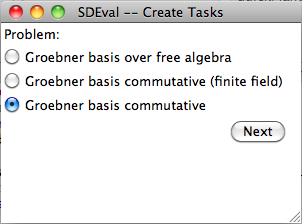
\includegraphics[width=0.5\textwidth]{pics/window1.png}
    \caption{Selection of the provided computation problems}
    \label{fig:window1}
\end{figure}

\newpage
You choose one, and click next. Then a window like in Figure \ref{fig:window2} appears.

\begin{figure}[ht]
    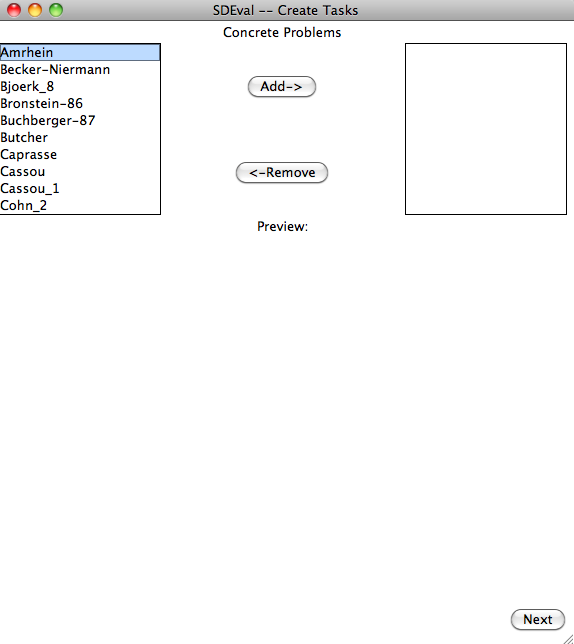
\includegraphics[width=1\textwidth]{pics/window2.png}
    \caption{Selection of problem instances from Symbolic-Data}
    \label{fig:window2}
\end{figure}

There, you can choose certain problem instances you want to have calculations to be run at. For a preview, simply double click on an entry in the left list box. If you want to add it, mark it and click the add button. Once you have selected all problem instances you want to use, click a last time on the ``Next''-Button.

\newpage
Then a window appears, where you can select different computer algebra systems. It looks like Figure \ref{fig:window3}.

Additionally, you have to add the commands to execute the selected computer algebra systems on your target machine. Also for a time command ist asked, which is on most \texttt{UNIX}-Like machines simply \texttt{time}. After giving your task a name, you can click on the ``Create''-Button, and then you will be asked where to save the taskfolder. Select a location. After that, the program creates a taskfolder in the specified path.

\begin{figure}[ht]
    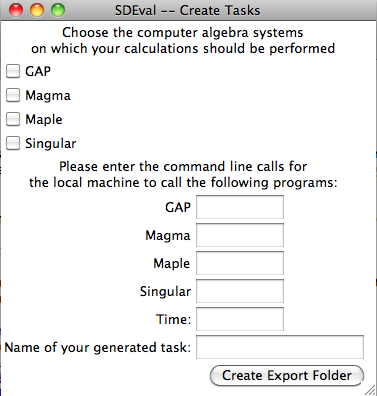
\includegraphics[width=1\textwidth]{pics/window3.png}
    \caption{Selection of computer algebra systems and setting the commands.}
    \label{fig:window3}
\end{figure}

\begin{remark}
  All those steps can also be done using the command line. For that, simply execute

\texttt{\$ python create\_tasks.py}
\end{remark}
\newpage
\subsection{Executing a Task}


Once you have created a task as described above, move to the taskfolder. There, you can execute the task by running the command

\texttt{\$ python runTasks.py}

\begin{remark}
  You can also add time constraints and memory usage constraints. You can find out how to do that by typing

\texttt{\$ python runTasks.py --help}
\end{remark}

After you do that, your computer seems to be working. But you do not know what it is doing. The answer is: It is executing all files on the corresponding computer algebra systems, which might take a while.

To see the proceedings of the computations, go into the subfolder \texttt{results}, which is created after the first running, and select the folder with the name representing the current timestamp. In there, you find a HTML-file called proceedings.html. Open it, and see which computations are waiting, running and which are completed.

For the completed, you can open resultedtimings.html, where you can see how long the calculation took.

That is it. Have fun using it!!!

\end{document}
